\chapter{Implementation}
\label{chap:impl}

\texttt{clerk} can be used to produce a styled spreadsheet with some data and formulas on it. These formulas are evaluated when the document is loaded into a target spreadsheet system.

The library supports the following features:

\begin{itemize}
  \item Typed cell references. Example: \texttt{Ref Double};
  \item Type-safe arithmetic operations with them. Example: \texttt{(a :: Ref Double) + (b :: Ref Double)} produces a \texttt{Ref Double};
 \item Constructing expressions with given types. Example: \texttt{("SUM" [a .: b]):: Expr Double} translates to \texttt{SUM(A1:B1)} (actual value depends on the values of \texttt{a} and \texttt{b});
  \item Conditional styles, formatting, column widths.
\end{itemize}

\Cref{sec:ex1} demonstrates the formula syntax and \Cref{sec:ex2} provides an example of working with the library's data types.

\section{Example 1. Formulas}
\label{sec:ex1}

This section demonstrates the formula syntax via several examples.

\subsection{Imports}

These are the necessary imports.

\begin{mycode}
import Clerk
import Data.Text (Text)
import ForExamples (mkRef, showFormula)
\end{mycode}

\subsection{Sample formulas}

Formulas consist of references, functions, and values.
Here, I pretend that there are values with given types and that I can get references to them. I compose formulas using these references.

\begin{mycode}
r1 :: Ref Int
r1 = mkRef 2 4

r2 :: Ref Int
r2 = mkRef 5 6

r3 :: Ref Double
r3 = mkRef 7 8

t1 :: Text
t1 = showFormula $ toFormula r2

-- >>>t1
-- "E6"

t2 :: Text
t2 = showFormula $ (r1 .* r2) .+ r1 .^ r2 ./ (ref r3)

-- >>>t2
-- "B4*E6+B4^E6/G8"
\end{mycode}

\section{Example 2. Multiplication Table}
\label{sec:ex2}

This section shows how to describe a spreadsheet with a multiplication table. The program should produce an \texttt{xlsx} file with a multiplication table. \Cref{fig:mult} demonstrates a desired multiplication table and \Cref{fig:mult_formulas} shows the underlying formulas.

\begin{figure}[h]
  \centering
  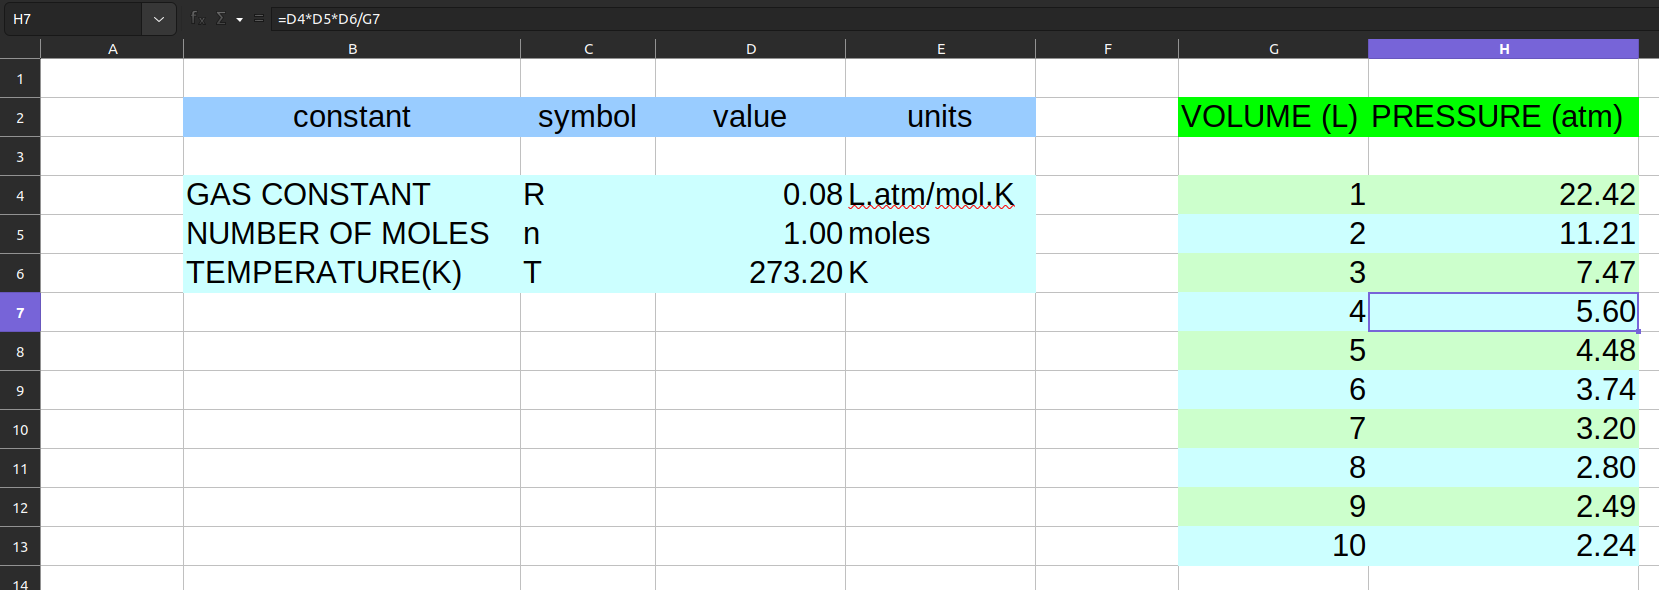
\includegraphics[scale=0.3]{demoValues.png}
  \caption{Multiplication table}
  \label{fig:mult}
\end{figure}


\begin{figure}[h]
  \centering
  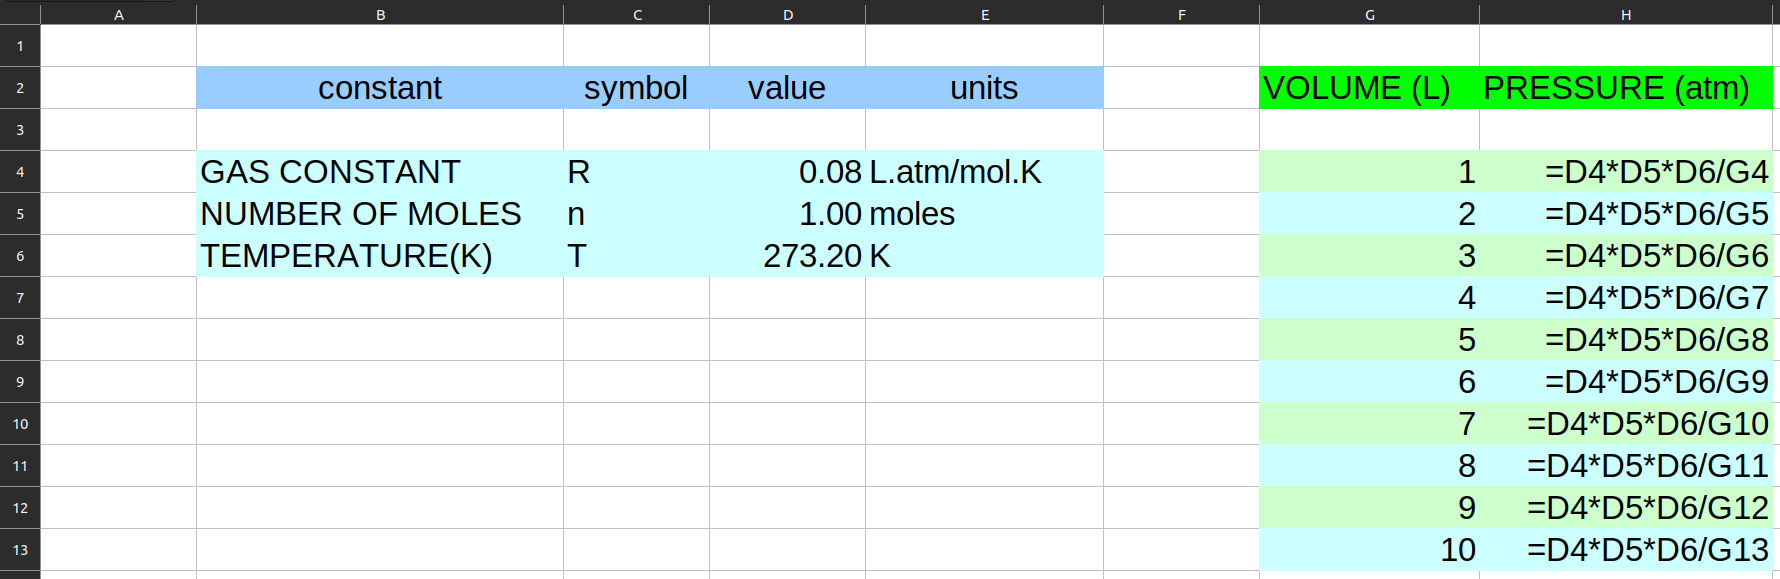
\includegraphics[scale=0.3]{demoFormulas.png}
  \caption{Multiplication table with formulas}
  \label{fig:mult_formulas}
\end{figure}


The below sections describe how such a spreadsheet can be constructed.

\subsection{Imports}

These are the necessary imports.

\begin{mycode}
import Clerk
import Control.Monad (forM, forM_, void)
import qualified Data.Text as T
import Lens.Micro ((&), (+~), (^.))
\end{mycode}

\subsection{Tables}

The tables that I construct are:

\begin{itemize}
  \item A vertical header;
  \item A horizontal header;
  \item A table with results of multiplication of the numbers from these headers.
\end{itemize}

\subsubsection{A vertical header}

\texttt{clerk} provides the \texttt{RowI} monad.
This monad takes some \texttt{i}nput, internally converts it into spreadsheet types, and outputs something, e.g., a cell reference.
In background, it writes a template of a horizontal block of cells - a \texttt{row}.
This row is used for placing the input values onto a sheet.

A vertical block of cells (\Cref{fig:vertical}) can be represented as several horizontal blocks of cells placed under each other.

\begin{figure}[h]
  \centering
  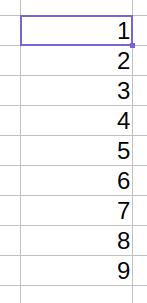
\includegraphics[scale=0.3]{vertical.png}
  \caption{A vertical header}
  \label{fig:vertical}
\end{figure}

As a template, I use a \texttt{RowI} with one integer as an input.
Because I do not need any formatting, I use \texttt{blank} cells for templates. I place the rows for each input value and collect the references.
Each row is shifted relative to the input coordinates.

\pagebreak

\begin{mycode}
mkVertical :: Coords -> [Int] -> Sheet [Ref Int]
mkVertical coords numbers =
  forM (zip [0 ..] numbers) $ \(idx, number) ->
    place1
      (coords & row +~ idx + 2)
      number
      ((columnRef blank (const number)) :: RowI Int (Ref Int))
\end{mycode}

\subsubsection{A horizontal header}

For a horizontal header (\Cref{fig:horizontal}), I make a row of numbers and collect the references to all its cells.

\begin{figure}[h]
  \centering
  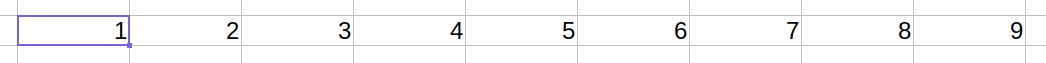
\includegraphics[scale=0.3]{horizontal.png}
  \caption{A horizontal header}
  \label{fig:horizontal}
\end{figure}

As the type of inputs is not important, I use the \texttt{Row} type.
In the \texttt{Sheet} monad, I place this row starting at a specified coordinate.

\begin{mycode}
mkHorizontal :: Coords -> [Int] -> Sheet [Ref Int]
mkHorizontal coords numbers =
  place
    (coords & col +~ 2)
    ((forM numbers $ \n -> columnRef blank (const n)) :: Row [Ref Int])
\end{mycode}

\subsubsection{Table builder}

For inner cells, I use single-cell rows for each input. I place the cells as in \Cref{fig:table}.

\begin{figure}[h]
  \centering
  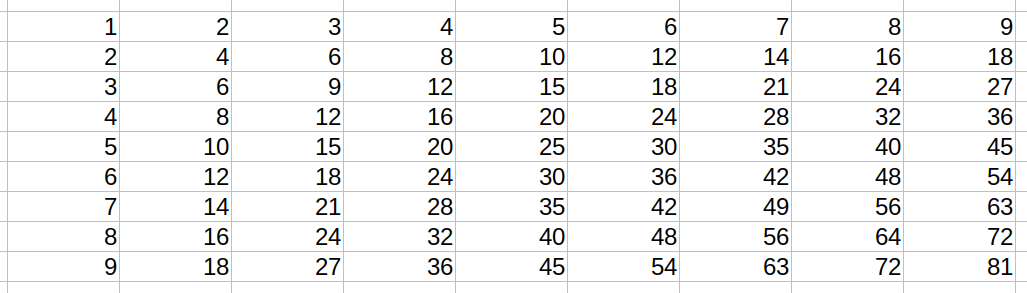
\includegraphics[scale=0.25]{table.png}
  \caption{A vertical header}
  \label{fig:table}
\end{figure}

\pagebreak
Since the information about these cells is unnecessary, I use the \texttt{Row ()} type.

\begin{mycode}
mkTable :: [(Ref Int, Ref Int)] -> Sheet ()
mkTable cs =
  forM_ cs $ \(r, c) -> do
    coords <- mkCoords (c ^. col) (r ^. row)
    place coords ((column blank (const (r .* c))) :: Row ())
\end{mycode}

\subsection{Sheet}

Here, I combine all functions to compose a complete \texttt{Sheet ()}.

\begin{mycode}
sheet :: Sheet ()
sheet = do
  start <- mkCoords 2 2
  let numbers = [1 .. 9]
  cs <- mkHorizontal start numbers
  rs <- mkVertical start numbers
  mkTable [(r, c) | r <- rs, c <- cs]
\end{mycode}

\subsection{Result}

Finally, I write the result and get a spreadsheet like the one at the beginning of this example.

\begin{mycode}
main :: IO ()
main = writeXlsx "example2.xlsx" [(T.pack "List 1", void sheet)]
\end{mycode}

% \begin{longtable}{c|c}
% \caption[This is the title I want to appear in the List of Tables]{Simulation Parameters} \label{table:fousimulation_params} \\
% \hline
% A & B  \\
% \hline
% \endfirsthead
% \multicolumn{2}{@{}l}{} \\
% \hline
% A & B \\
% \hline
% \endhead
% \hline
%  \textbf{Parameter} & \textbf{Value}\\
%  \hline
%  Number of vehicles & $|\mathcal{V}|$\\
%  \hline
%  Number of RSUs & $|\mathcal{U}|$\\
%  \hline
%  RSU coverage radius & 150 m\\
%  \hline
%  V2V communication radius & 30 m\\
%  \hline
%  Smart vehicle antenna height & 1.5 m\\
%  \hline
%  RSU antenna height & 25 m\\
%  \hline
%  Smart vehicle maximum speed & $v_{max}$ m/s\\
%  \hline
%  Smart vehicle minimum speed & $v_{min}$ m/s\\
%  \hline
%  Common smart vehicle cache capacities & $[50, 100, 150, 200, 250]$ mb\\
%  \hline
%  Common RSU cache capacities & $[5000,1000,1500,2000,2500]$ mb\\
%  \hline
%  Common backhaul rates & $[75, 100, 150]$ mb/s\\
%  \hline
% \end{longtable}

% \begin{figure}[hbt]
% \centering
% 
\includegraphics[]{figs/inno.png}
% \caption{One kernel at $x_s$ (\emph{dotted kernel}) or two kernels at
% $x_i$ and $x_j$ (\textit{left and right}) lead to the same summed estimate
% at $x_s$. This shows a figure consisting of different types of
% lines. Elements of the figure described in the caption should be set in
% italics, in parentheses, as shown in this sample caption.}
% \label{fig:fouex}
% \end{figure}

% \ldots
